%2345678901234567890123456789012345678901234567890123456789012345678901
\chapter{Introduction}
\label{introduction}

\section{Technical development of astronomy} % (fold)
\label{sec:astronomy_technical_developments}
	
	Astronomy has always been a technology enabled science. The sky
	was well known to the ancient cultures who found it a source for
	their calendaring systems, which allowed them to predict floods,
	find the best time of the year for seeding, and even reinforce
	the status of religious ministers due to their connection to the
	universe. But even that early astronomy demanded accurate
	instruments for timekeeping, angle measurement, and building
	alignment to mark specific parts of the year thanks to the
	motion of the sun in the sky throughout the year.
	
	 It was not until the times of Galileo, the first historically
	acknowledged user of a telescope, that astronomy suffered
	another impulse. The discovery of the Galilean moons revolving
	around a celestial body other than the Earth put an end to the
	Ptolemaic illusion that everything in the sky revolved around
	the Earth, and helped establishing the Copernican paradigm
	shift, where our planet was no longer the centre of the known
	universe. That shift renewed the interest in astronomy, and
	thanks to it the orbits of planets were determined, larger and
	better telescopes were built to find fainter objects, and more
	planets and moons were found.
	
	 The next leap in astronomy was the invention of spectroscopy,
	together with the recognition of \emph{fingerprints} of elements
	in the spectra, which for the first time allowed us to know what
	August Comte had thought impossible to learn: what was the
	constitution of \emph{heavenly bodies}\footnote{Comte wrote:
	\emph{The mathematical thermology created by Fourier may tempt
	us to hope that, as he has estimated the temperature of the
	space in which we move, we may in time ascertain the mean
	temperature of the heavenly bodies: but I regard this order of
	facts as for ever excluded from our recognition. We can never
	learn their internal constitution, nor, in regard to some of
	them, how heat is absorbed by their atmosphere. We may therefore
	define Astronomy as the science by which we discover the laws of
	the geometrical and mechanical phenomena presented by the
	heavenly bodies.}}~\cite{1896psac.book..149C}. Not only that,
	but spectroscopy can tell us what the physical conditions inside
	a remote part of the universe are like. This development was so
	important that even astronomy changed its name, becoming
	astrophysics. We must also remember that for most celestial
	bodies our only source of information is the light\footnote{In
	this thesis, we will use \emph{light} to refer to all kinds of
	detectable electromagnetic radiation, from the radio band to the
	gamma rays, and when referring specifically to visible
	electromagnetic radiation, which our eyes can perceive, we will
	always use the \emph{visible} adjective.} they emit, absorb,
	eclipse or otherwise affect. It is the careful treatment of such
	light, together with the always improving knowledge of the
	physical processes affecting it what allows us to recover from
	that electromagnetic radiation large amounts of information from
	extremely distant and dim objects.
	
	 Learning how to permanently register light was first achieved
	in 1826 by Nicéphore Niépce, and a more repeatable and faster
	process was announced by Louis Daguerre in 1839, who took
	himself the first photograph of the Moon during that very
	year~\cite{1961apdt.book.....D, Abrahams:kc}. Just in 1843 the
	process is applied for the first time to the spectrum of the sun
	by J.W. Dapper, leading to the discovery of new lines in
	ultraviolet wavelengths, long before Bunsen and Kirchhoff showed
	that those lines were due to absorption by several atomic
	species. Photography made astrophysics a truly experimental
	science, as spectra could be now recorded and compared between
	observations.
	
	 Another breakthrough in astronomy came hand in hand with a new
	technology: the discovery of extraterrestrial radio signals by
	Karl Janksy in 1933, for which he tried to fix a position that
	seemed to be coincidental with the centre of our own
	galaxy~\cite{Jansky:1933db, Jansky:1935lq}. This opened a new
	window for astrophysics, as the radio sky seemed at first very
	different, almost unrelated to the visible sky, and many
	different objects were discovered, such as pulsars, quasars,
	galactic jets, et cetera. One of the most relevant new insights
	for cosmology was the discovery of the Cosmic Microwave
	Background radiation by Penzias and
	Wilson~\cite{1979Sci...205..866W, 1979Sci...205..549P}, which
	backed our current \emph{Big Bang} model of our Universe.

\begin{figure}[tbp]
	\centering
		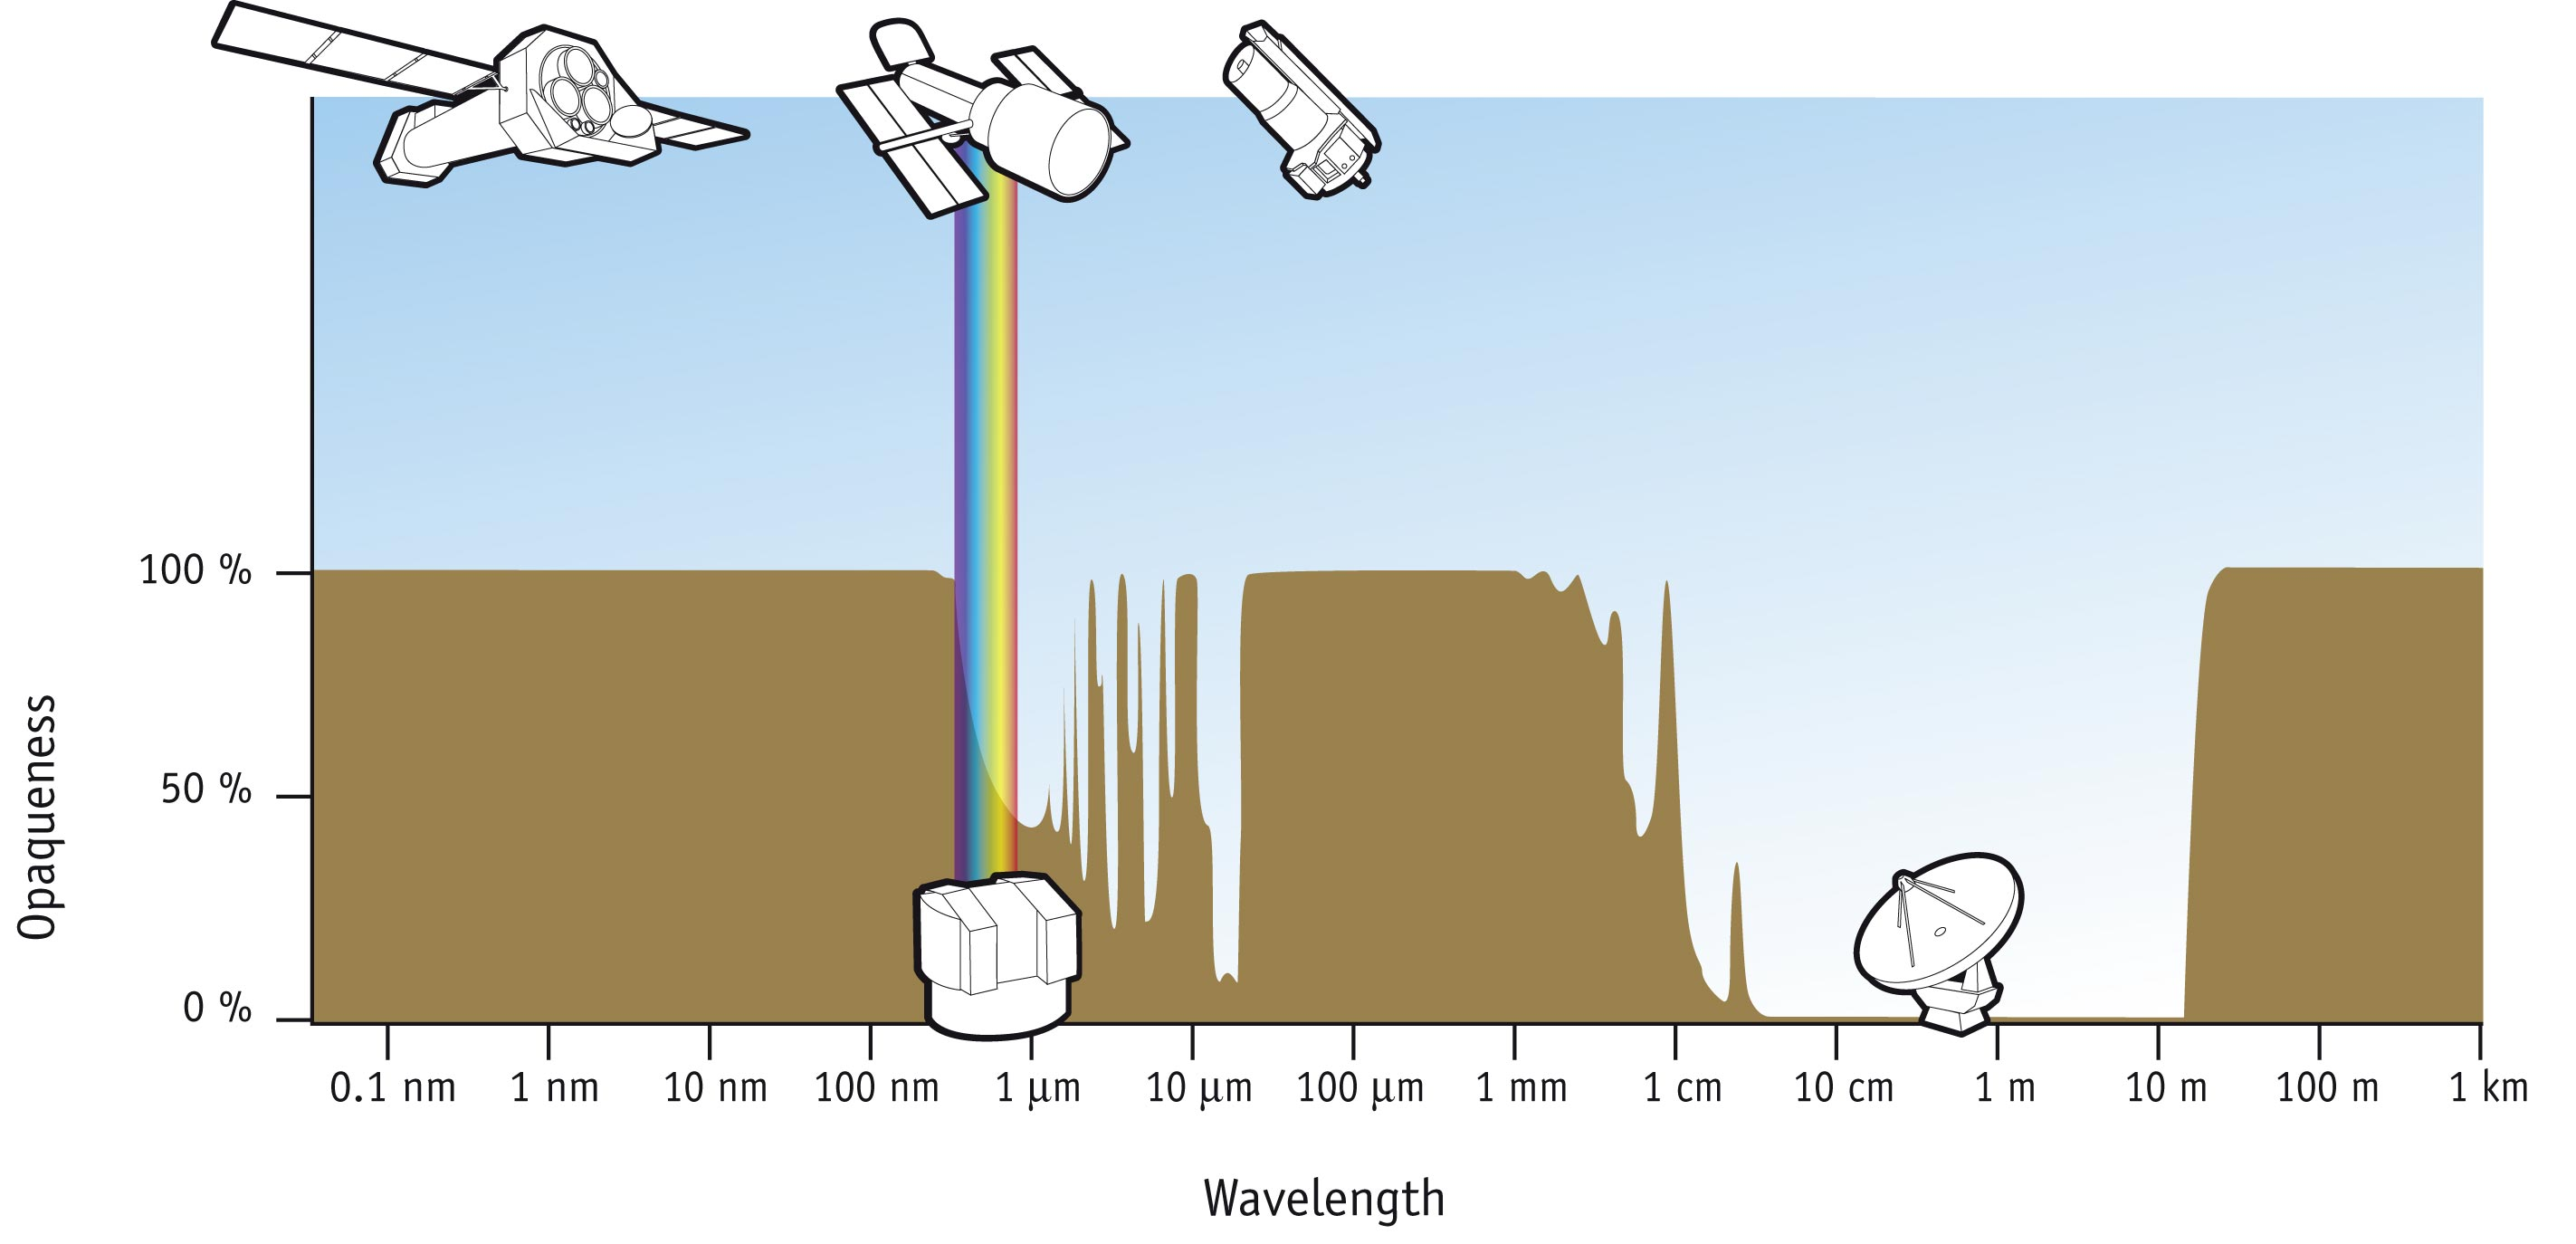
\includegraphics[width=\columnwidth]
		{fig/AtmosphericOpaquenessVsWavelength.png}
	\caption[Atmospheric opaqueness versus wavelength.]
	{
		Atmospheric opaqueness as a function of wavelength. Earth's
		atmosphere is opaque to most electromagnetic radiation,
		except for the visible window, which reaches from the
		near-infrared to the near (soft) ultraviolet radiation.
		There is also a radio window for electromagnetic radiation
		with wavelengths between 1~mm and several tens of meters,
		and it is not totally opaque for radiation above the $1/10$
		of a millimetre. The main responsible for atmospheric
		absorption of sub-mm radiation is water vapour, and dry
		regions such as those in the South Pole or in the Atacama
		Desert can be used for observations in the sub-mm range.
		This image was created for NASA by STScI under Contract
		NAS5-26555 and for ESA by the Hubble European Space Agency
		Information Centre, and is in the public domain.
	}
	\label{fig:fig_AtmosphericOpaquenessVsWavelength}
\end{figure}

	 Then came the new windows opened when the space career
	started, allowing humankind, for the first time, to have
	observatories outside of the atmosphere, which is opaque for
	radiation other than radio and visible light ---see
	figure~\ref{fig:fig_AtmosphericOpaquenessVsWavelength}---. We
	were rewarded with the discovery of strong X-ray sources marking
	active galaxy nuclei, supernovae, and the incredibly bright and
	distant Gamma-Ray Bursts. By being free of the atmosphere, the
	Hubble Space Telescope has provided us with the deepest view of
	our Universe, thanks to the repeated, accumulated exposure of
	the Ultra Deep Field~\cite{2006AJ....132.1729B}.
	
	 Of course, our current observatories, both ground-based and
	space-borne, have only been possible after Charge Couple
	Devices (CCDs) started to replace photographic plates. The
	sensibility of CCDs (measured as their quantum efficiency, or
	percentage of times a photon incidence produces a measurable
	change in the sensing element) is much superior to that of
	photographic plates, allowing the detection of fainter
	objects. Besides, several other capabilities, specially direct
	electronic output and linearity in their response, make them
	much more desirable than film for scientific, and particularly
	astronomical purposes.

% section astronomy_technical_developments (end)

\section{Astronomy data today} % (fold)
\label{sec:astronomy_today}

	%	\begin{figure}[tbp]
	%		\centering
	%			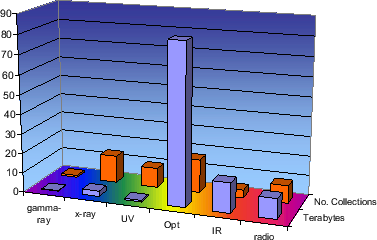
\includegraphics[width=\columnwidth]{fig/img7.png}
	%		\caption{caption}
	%		\label{fig:fig_img7}
	%	\end{figure}

	Contemporary astronomy is built around the idea of digitised
	observations. Everything is quantised, digitised, and processed
	using digital computers, something made easier by the digital
	nature of CCDs.
	
	 This digital nature makes it more natural to mix datasets from
	different observatories, giving birth to what is called
	multiwavelength astronomy. By combining the light received from
	as many instruments as possible, we can learn an increasing
	number of properties of distant objects. For instance, we can
	try to fit spectral models to the actually recorded spectrum,
	being that fitting more reliable when considering the most
	bands.
	
	 Building that multiwavelength picture is, nevertheless, not
	trivial. Astronomers need to perform their own observations
	of the objects of their interest with many different
	observatories and instruments, something very costly in terms
	of both time (observation proposals have to be written, and if
	approved then the actual observation has to be performed,
	processed, and analysed) and effort (spent in learning the
	different packages needed to reduce astronomical data from
	different observatories); or instead, astronomers can rely on
	observations previously performed by other astronomers, and
	stored in the archive of observatories of their interest.
	
	 In any case, very few observatories have archives, and
	those which have them provide datasets with very different
	science requirements. Some observatories provide raw data,
	which have to be combined with calibration data for the
	astronomer to perform the data reduction, while others provide
	already reduced data products with very little information on
	how that reduction was performed, which were the observing
	conditions, and so on. Each different archive is accessed
	through its own access portal, has different access policies,
	different data browsing mechanisms, and data are finally
	delivered in different formats. And there is the additional
	issue of finding out which archives exist which carry data of
	our interest.
	
	 An interesting exception to the lack of archives are
	space-borne observatories. These facilities are so expensive,
	essentially due to the launching costs,\invisiblenote{but also
	to the research and development invested into the satellite,}
	that collected data have to be made available to the community
	after typically one year of proprietary period in order to
	maximise the scientific return from their observations. The
	cost of the archive is a small fraction of the operational cost
	for the mission, and all space satellites provide some sort of
	access to their archives. The kind of data products provided by
	each mission, however, is not standardised, either.

	\invisiblenote{
	 In the late seventies, the use of digitised imaging, and the
	need of computer-intensive Fast Fourier Transforms for imaging
	in radio interferometry made several institutions create, in
	the late seventies, a common Flexible Image Transport System,
	the FITS file format. That data format was presented to the
	community in 1981~\cite{1981A&AS...44..363W}, and solved part
	of the problem of image (and spectral, and tabular data)
	transport, but the flexibility of the system made FITS files
	not fully compatible between different software packages.
	}
	
	%	\footnote{To be fair, astronomy has had since the 70's a common
	%	data format, the Flexible Image Transport System (FITS), to
	%	which most archives and instruments adhere. However, the
	%	complexity of many astronomical observations allow for very
	%	different layouts of the data, and FITS headers are not always
	%	easy to read for a machine in order to interpret available
	%	data.}.

	 A third source of data for the astronomer are large sky surveys,
	which have started to take place in the last few years, in which
	data are collected by dedicated wide-field telescopes, with
	reduction pipelines working for several spectral bands. The
	pipelines perform digital processing on the images, and
	determinate tens or hundreds of properties for selected objects.
	Such is the case of recent surveys, such as the Sloan Digital
	Sky Survey (SDSS)~\cite{1995wfsd.conf....3G,
	2000AJ....120.1579Y}, such as the Two Micron All Sky Survey
	(2MASS)~\cite{2006AJ....131.1163S}, but also for the digitised
	version of the Second Palomar Observatory Sky Survey (POSS-II,
	D-POSS), or even the older, National Geographic Society-Palomar
	Observatory Sky Survey (NGS-POSSdigitised).

	% Remember, the Digitised POSS-I conforms
	% the Digitised Sky Survey,
	% base of the Microsoft World Wide Telescope,
	% y de Google Sky.

	 Not all surveys are optical, and there are radio surveys such
	as the the FIRST~\cite{1994ASPC...61..165B} and
	NVSS~\cite{1993BAAS...25.1389C} surveys, performed with the
	Very Large Array radio interferometer (VLA), or the
	ALFALFA~\cite{2008arXiv0806.1670H, 2005AJ....130.2598G}, being
	performed with the Arecibo radio telescope.
	
%	The problem the astronomer faces today is twofold:
%	
%	\begin{itemize}
%		\item how to retrieve everything that is available from all
%        the different archives, in order to know whether he needs to
%        apply for observation time or not; and
%		
%		\item how to access all information at the same time in
%        order to derive statistical properties.
%	\end{itemize} 
%	
%	This last point is of the utmost importance for extragalactic
%    astronomy, given than most galactic processes have time scales
%    of giga-years, and in that case we are looking essentially at a
%    snapshot of the universe. If we want to derive properties, we
%    need to compile statistics for objects of the same kind, but for
%    those statistics to be meaningful we need to use very large
%    samples. And for those large samples to be built we need to
%    access a large amount of archives whose organisation (as of now)
%    is completely different, and whose access interfaces were
%    thought for the individual astronomer, not for direct machine
%    interrogation.

% section astronomy_today (end)

\section{Astronomical archives: benefits and problems} % (fold)
\label{sec:astronomical_archives}

	As pointed in the section before, self-performed observations
	are but one of the ways for astronomers to collect data
	relevant to their research, while data archives, be them
	originated from the systematic storage of observational data
	from each telescope and instrument, from broad sky surveys, or
	from space-borne missions, conform nowadays the main resource
	of astronomical data.
	
	 Archives provide several benefits for astronomers:

	\begin{description}
		\item[Efficiency in resource usage] If the observation an
		astronomer wishes to perform has already been made, there
		is no need to go through the full process of writing
		observation proposals or to wait for the allocated time.
		The data can be downloaded by many different users, serving
		many different purposes, some perhaps never considered at
		the time of the observation.
		
		\item[Time domain exploration] Some astronomical objects
		have properties varying in time. Comparing observations
		taken in different moments allows to study periodic
		phenomena (variable stars, asteroid rotation, pulsars, et
		cetera), or transient phenomena (novae and supernovae,
		Gamma-Ray Bursts, et cetera)
		
		\item[Statistical inference] Most astronomical processes %
		(specially those regarding extra-galactic astronomy) have
		time scales much larger than our civilisation life-span,
		and our only way to explore them is to take into account as
		many objects of the same type as possible. This includes
		defining object types, something which can be simplified by
		data mining techniques, which in turn require large
		datasets to explore.
		
		\item[Non-exclusive access] Public archives allow
		astronomers from countries with limited research resources
		to access high-quality data, and produce top-level science.
	\end{description}

	However, in their current incarnation, archives pose several 
	problems:

	\begin{description}
		\item[Ever increasing datasets] There is no way to know when
		a particular observation will be useful, so all observations
		must be stored, and together with them all the ancillary
		data (weather conditions, seeing, opacity, telescope
		orientation, instrumental calibration observations, et
		cetera) needed to reduce the raw observation data in order
		to get scientific data products. That means every year
		archives have to manage more and more data. An example can
		be seen in figure~\ref{fig:fig_ESODataHoldings}.
		
		 \item[Ever increasing dataset size] Telescopes are built
		with 25 to 50 years life-spans, but instruments are changed,
		improved, and added, so that the same telescope can provide
		more and more resolution and sensitivity over the years, as
		CCDs tend to follow Moore's Law~\cite{1965E......38.....M},
		and double every two years ---see
		figure~\ref{fig:fig_CCDresolutionIncrease}---. That makes
		each dataset to be archived larger for each new facility or
		instrument.
		
		 \item[Ever improving data reduction techniques] The actual
		data being collected are in the form of voltages, or
		detection counts, that have to be converted in physical
		magnitudes such as temperature, emitted energy, mass, et
		cetera, which can be derived thanks to the knowledge of all
		the physical processes affecting the measurement, but also
		to a very careful measurement of observational effects. When
		the technical knowledge of those effects improves, many
		archives provide a new version of the derived data,
		contributing both to the data increase, but also to the need
		to document how each version has been obtained.
		
		 \item[Non-uniform, non-centralised access] Nowadays, most
		instrumental archives are accessible via internet, but each
		different telescope ---or even each different instrument---
		has a different web portal, with different query parameters,
		which are difficult to access in an automated way. Besides,
		there is no way for an astronomer ---much less so for a
		software system--- to learn when a particular archive, or
		data set within that archive, has been released, as many
		observations are held for a certain \emph{proprietary
		period} during which the original observer has exclusive
		access to it.
	\end{description}

	\begin{figure}[btp]
		\centering
		%\includegraphics[width=0.8\columnwidth]
		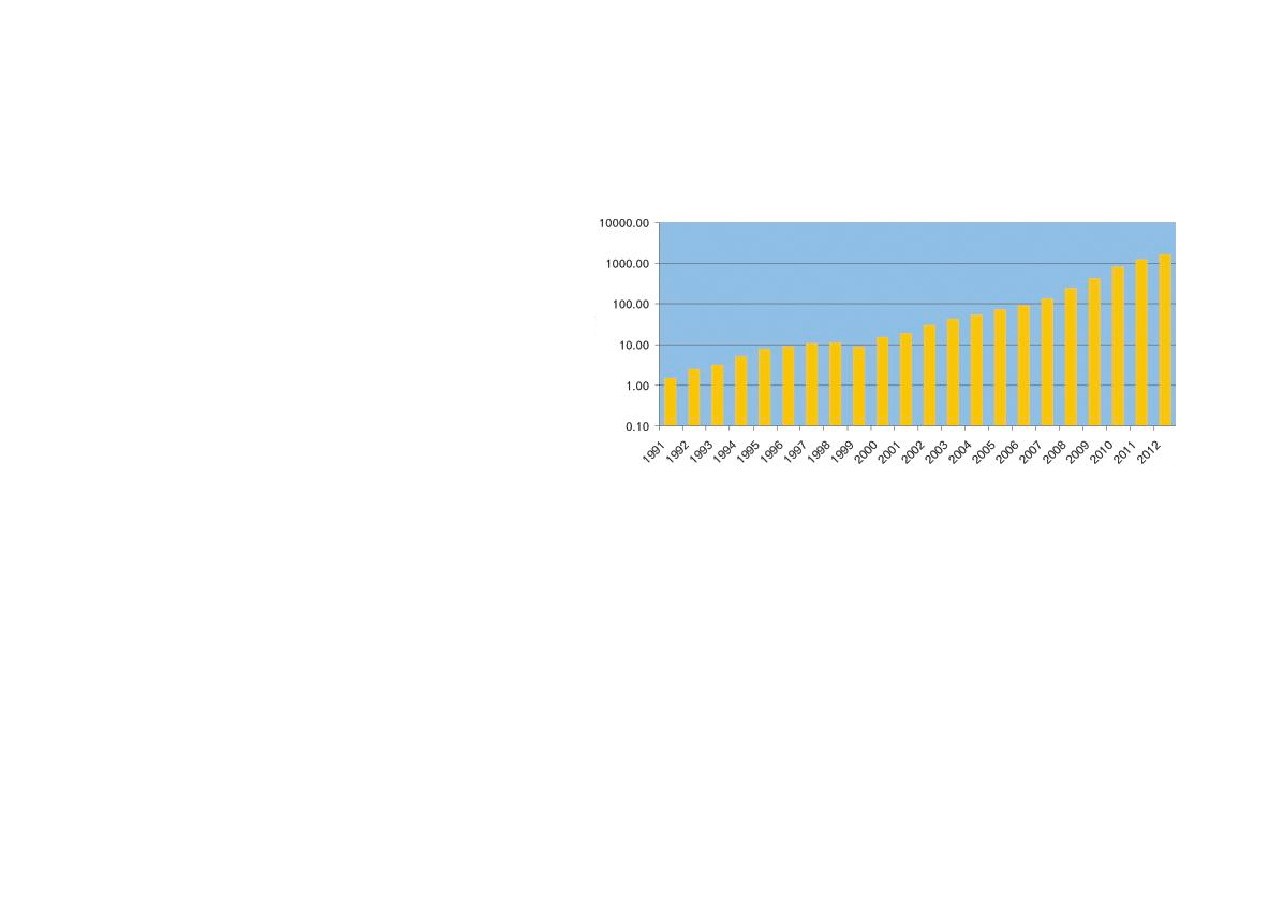
\includegraphics[scale=1]
				{fig/ESODataHoldings.pdf}
		\caption[Evolution of the
		         ESO data holdings]
		{
			Evolution of the amount of data stored in the ESO
			archive since 1991 to 2003 (in Terabytes in logarithmic
			scale), together with predictions till 2012.
			Reproduced from~\cite{ESO:2003la}.
		}
		\label{fig:fig_ESODataHoldings}
	\end{figure}

	\begin{figure}[btp]
		\centering
		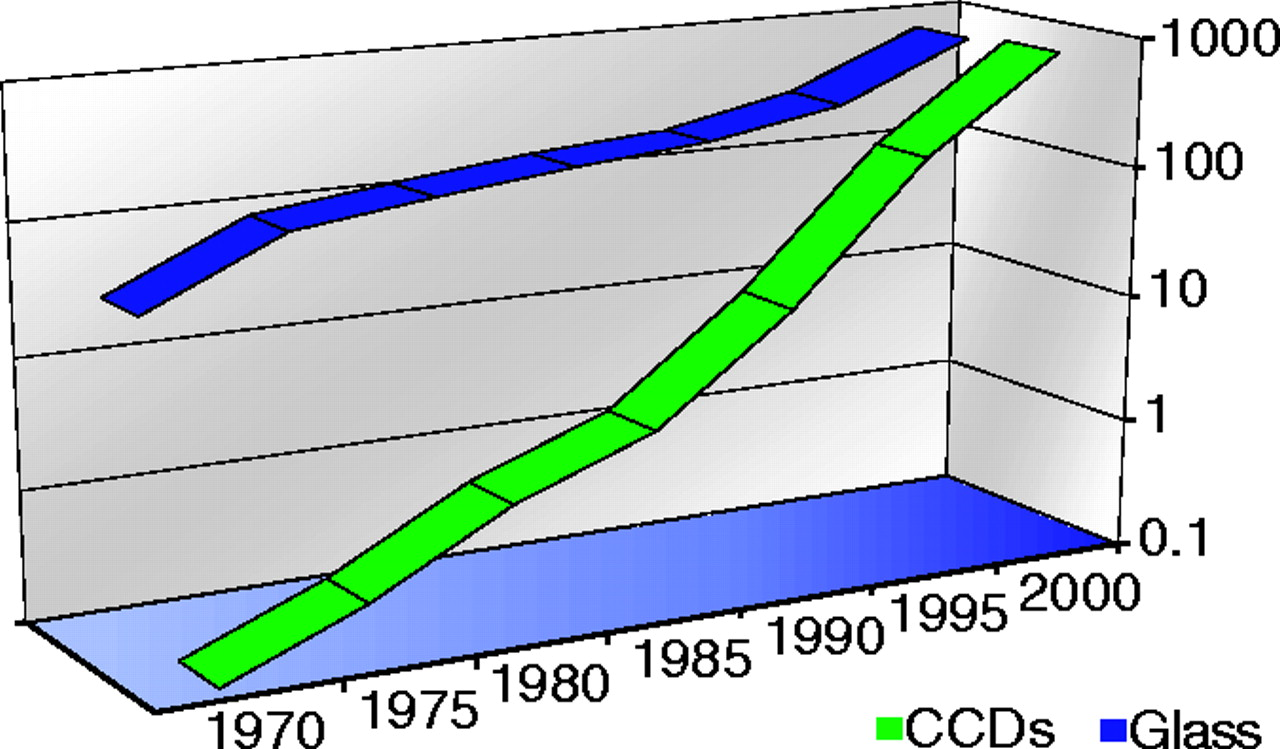
\includegraphics[width=0.8\columnwidth]
		     {fig/CCDresolutionIncrease.jpg}
		\caption[Evolution of telescope areas and CCD pixel resolution]
		{
			Telescope collecting surface area (labelled Glass) and
			CCD pixel resolution in logarithmic scale versus linear
			time since 1970 (arbitrary units). It can be seen that
			CCDs, governed by \glossaryentry{Moore's Law}, have a
			much steeper increase rate, doubling roughly every 2
			years, whereas telescope area doubles every 25 years.
			Reproduced from~\cite{2001Sci...293.2037S}.
		}
		\label{fig:fig_CCDresolutionIncrease}
	\end{figure}

	 Thus, astronomers in the era of archives face the following
	problems:

	\begin{itemize}
		\item finding out and retrieving already available data from
		existing archives, remaining aware of additional datasets
		which might be released at any time;
		
		 \item combining datasets from different archives in a
		sensible way;
		
		 \item managing huge datasets simultaneously in order to
		derive statistical properties;
		
		 \item performing analysis of large datasets on a
		distributed system; this problem is compounded by the
		bottleneck of network bandwidth, which not increasing at the
		same rate as the astronomical data set size.
	\end{itemize}

	A suitable solution for those issues, then, should provide:

	\begin{itemize}
		\item Mechanisms for finding each and every data repository
		available in each moment must exist.
		
		 \item Complete descriptions of each data repository, so
		that those not containing data of interest for the
		astronomer ---as specified by several selection criteria,
		such as wavelength or resolution--- can be filtered out.
		
		 \item Unified data description and format, so that data
		coming from heterogeneous sources can be easily combined,
		and operated with.
		
		 \item Minimum data transfer between users of archived data
		and the data; data processing must be moved preferentially
		to the server, and only processed data should be sent back
		to the astronomer.
	\end{itemize}

	Such a system would provide each astronomer in the world with a
	virtual observing facility able to picture the sky in all the
	wavelengths at the same time, without the need for the
	astronomer to manually discover each of the datasets which will
	conform that picture, or to perform conversions on data coming
	from different instruments. That system exists, and is called
	the Virtual Observatory.
	
	 Discussions on the Virtual Observatory concept were started
	with the \emph{Virtual Observatories of the
	future}~\cite{2001ASPC..225.....B}
	and \emph{Mining the sky}~\cite{2001misk.conf..674G}
	conferences, held
	in 2000 at Caltech and Garching bei Müenchen, respectively.
 	The north american
	National Virtual Observatory project started in 2001 with a 
	10 million dollar funding, and 17 centres involved. Finally,
	Jim Gray and Alex Szalay summarised and generalised the concept
	in their 2001 article \emph{The World-Wide
	Telescope}~\cite{2001Sci...293.2037S} in \emph{Science}, and the
	community
	started prototyping the system in 2002.
	
	 However, many different \emph{virtual observatories} can be
	built following the previous definition.
	In order to have a single
	Virtual Observatory where all datasets and tools are
	interoperable, standards need to be set and adhered to. Thus a
	standards sanctioning body is needed, and that is the role of
	the International Virtual Observatory Alliance (IVOA).
	
	 The VO is still in development, but nearing what is called the
	\emph{operations stage}, where astronomers are regularly using
	VO tools for their research. However, in this thesis will see
	that there are several problems with the current incarnation of
	the VO, particularly in the scope of radio astronomy, and
	multidimensional data access.
	
	In Spain, the national VO initiative is the Spanish Virtual
	Observatory (SVO), which joined the IVOA in 2004, and which is
	focused in promoting science with the VO in Spanish astronomy,
	and in providing specific tools for performing that science.
	
	We wish to emphasise that this is the first technical thesis
	developed within the SVO framework.

% section astronomical_archives (end)

\section{Thesis aim} % (fold)
\label{sec:thesis_aim}
	
	This thesis is devoted to the study of:

	\begin{description}
	
		\item [The VO infrastructure] Which are the components of
		the VO, and which are the interfaces to them, with special
		emphasis on missing or underdeveloped blocks for radio
		astronomical data. This is the scope of
		chapter~\ref{intro_vo} of Part~\ref{prt:intro_vo}.
	
		 \item[Modelling radio astronomical data] For radio
		astronomical data to be properly described within the VO
		data models are needed. Part~\ref{partRadioDataModelling} is
		devoted to the RADAMS, the data model developed for radio
		astronomical observations.
	
		 \item [Bringing legacy tools to the VO] As there are many
		man-years of experience invested in many already existing
		astronomical tools, we will study how to incorporate those
		tools into the VO ecosystem. We have developed a Modular VO
		Interface for Radioastronomy (MOVOIR) which provides both a
		GUI for accessing the VO, and tools for adapting legacy
		tools to use VO protocols. Part~\ref{prt:legacyTools} is
		devoted to it.
	
		 \item [Applied work] We have used the RADAMS data model as
		the basis for the astronomical archives of the IRAM~30m and
		DSS-63~70m radio telescopes, and the MOVOIR as the basis for
		bringing the \massa{} and \madcuba{} legacy
		applications into the VO. We show our results in
		Part~\ref{prt:thesis_applications} is devoted to the
		archives which have been built using the RADAMS.
	
	
	\end{description}

	As a result of this study, complete VO-compliant radio astronomy
	model has been created, two astronomical archives have been
	implemented, and a software tool has been developed for allowing
	legacy radio astronomical tools access the VO.

% section thesis_aim (end)


\section{Thesis context} % (fold)
\label{sec:thesis_context}

	This thesis work has been developed and written
	\invisiblenote{not
	within a computer science research group, but} within an
	astrophysical research project
	(AMIGA\urlnote{http://amiga.iaa.csic.es/}, Analysis of the
	interstellar Medium of Isolated GAlaxies) whose objective is
	studying a sample of isolated galaxies, with more than 1000
	members. A special emphasis is given on radio observations in
	the centimetre, millimetre, and sub-millimetre wavelength ranges
	because the (sub)mm spectral band delivers fundamental
	information to learn about physicochemical processes in the
	interstellar medium (ISM). It is relevant to note that astronomy
	in the (sub)mm range is suffering a strong technological
	advance, with new astronomical facilities, such as the
	Sub-Millimetre Array\urlnote{http://sma1.sma.hawaii.edu/} (SMA),
	and the well-advanced construction of the Atacama Large
	Millimetre Array\urlnote{http://almaobservatory.org/} (ALMA).
	
	 As public data access in the radio wavelength is limited, we
	had resolved to contribute in the building of radio data
	archives, working together with the IRAM to provide an archive
	for the IRAM 30m antenna. In parallel, we also undertook the
	development of the scientific archive for spectroscopic
	observations of the DSS-63 70m antenna at Robledo de Chavela,
	part of NASA's Deeps Space Network.
	
	\newcommand{\massaurl}[0]
	{http://damir.iem.csic.es/mediawiki-1.12.0/index.php/Portada}
	 Since our group does intensive analysis of 3D data at all
	wavelengths (in fact the current trend in spectroscopy), we
	also decided to collaborate in bringing existing software
	packages to solve the mentioned tasks, in order to make our
	research work more efficient. We have collaborated with Jesús
	Martín-Pintado's group at the Molecular and Infrared
	Astrophysics Department (DAMIR) of the Institute of Matter
	Structure, developers of the MASSA (MAdrid Single Spectrum
	Analysis) and \madcuba{} (MADrid CUBe Analysis)
	tools\footnote{Project wiki: \url{\massaurl}} for the Heterodyne
	Instrument for the Far
	Infrared\urlnote{http://www.sron.nl/divisions/lea/hifi/} (HIFI)
	of the soon to be launched Herschel
	spacecraft\urlnote{http://herschel.esac.esa.int/}, in order to
	make both tools compatible with the VO.
	
	 All the problems we need to solve are very similar to those of
	the astronomical community at large (save the emphasis in the
	radio band), namely:

	\begin{itemize}
		\item easy-to-use data look-up tools, in order to get
		multi-wavelength data for every object, to be retrieved from
		online archives;
		
		\item data combination tools, taking into account different
		data formats, coordinate systems, file metadata;
		
		\item physical parameter extraction tools: each different
		parameter must include different physics, and needs its own
		interface.
	\end{itemize}

	The community had already started to provide an
	information-technology-based solution: the Virtual Observatory.
	All the work performed for this thesis has been built within
	that framework, and in collaboration with the Spanish Virtual
	Observatory initiative.
	
% section thesis_context (end)

